\documentclass[10pt]{beamer}\usepackage[]{graphicx}\usepackage[]{color}
%% maxwidth is the original width if it is less than linewidth
%% otherwise use linewidth (to make sure the graphics do not exceed the margin)
\makeatletter
\def\maxwidth{ %
  \ifdim\Gin@nat@width>\linewidth
    \linewidth
  \else
    \Gin@nat@width
  \fi
}
\makeatother

\definecolor{fgcolor}{rgb}{0.345, 0.345, 0.345}
\newcommand{\hlnum}[1]{\textcolor[rgb]{0.686,0.059,0.569}{#1}}%
\newcommand{\hlstr}[1]{\textcolor[rgb]{0.192,0.494,0.8}{#1}}%
\newcommand{\hlcom}[1]{\textcolor[rgb]{0.678,0.584,0.686}{\textit{#1}}}%
\newcommand{\hlopt}[1]{\textcolor[rgb]{0,0,0}{#1}}%
\newcommand{\hlstd}[1]{\textcolor[rgb]{0.345,0.345,0.345}{#1}}%
\newcommand{\hlkwa}[1]{\textcolor[rgb]{0.161,0.373,0.58}{\textbf{#1}}}%
\newcommand{\hlkwb}[1]{\textcolor[rgb]{0.69,0.353,0.396}{#1}}%
\newcommand{\hlkwc}[1]{\textcolor[rgb]{0.333,0.667,0.333}{#1}}%
\newcommand{\hlkwd}[1]{\textcolor[rgb]{0.737,0.353,0.396}{\textbf{#1}}}%
\let\hlipl\hlkwb

\usepackage{framed}
\makeatletter
\newenvironment{kframe}{%
 \def\at@end@of@kframe{}%
 \ifinner\ifhmode%
  \def\at@end@of@kframe{\end{minipage}}%
  \begin{minipage}{\columnwidth}%
 \fi\fi%
 \def\FrameCommand##1{\hskip\@totalleftmargin \hskip-\fboxsep
 \colorbox{shadecolor}{##1}\hskip-\fboxsep
     % There is no \\@totalrightmargin, so:
     \hskip-\linewidth \hskip-\@totalleftmargin \hskip\columnwidth}%
 \MakeFramed {\advance\hsize-\width
   \@totalleftmargin\z@ \linewidth\hsize
   \@setminipage}}%
 {\par\unskip\endMakeFramed%
 \at@end@of@kframe}
\makeatother

\definecolor{shadecolor}{rgb}{.97, .97, .97}
\definecolor{messagecolor}{rgb}{0, 0, 0}
\definecolor{warningcolor}{rgb}{1, 0, 1}
\definecolor{errorcolor}{rgb}{1, 0, 0}
\newenvironment{knitrout}{}{} % an empty environment to be redefined in TeX

\usepackage{alltt}
\usetheme{metropolis}           % Use metropolis theme

\usepackage{graphicx}

\DeclareGraphicsExtensions{.pdf,.jpeg,.jpg,.png}

\usepackage{subcaption}
\usepackage{amsmath}

\usepackage{tikz}
\usetikzlibrary{bayesnet}
\usepackage{pgfplots}
\pgfplotsset{compat=1.13}

\usepackage[framemethod=TikZ, xcolor=RGB]{mdframed}
\definecolor{mydarkblue}{rgb}{0,.06,.5}
\definecolor{mydarkred}{rgb}{.5,0,.1}
\definecolor{myroyalblue}{rgb}{0,.1,.8}
\mdfdefinestyle{MyFrame}{%
    linecolor=mydarkblue,
    outerlinewidth=0.5pt,
    roundcorner=2pt,
    innertopmargin=2pt,
    innerbottommargin=2pt,
    innerrightmargin=2pt,
    innerleftmargin=2pt,
    backgroundcolor=blue!10}

\newcommand{\Rbb}{\mathbb{R}}
\newcommand{\Expect}{\mathbb{E}}
\newcommand{\Expecthat}{\hat{\mathbb{E}}}
\newcommand{\Var}{\text{Var}}
\newcommand{\Cov}{\text{Cov}}
\newcommand{\vbfamily}{\mathcal{Q}}
\newcommand{\etaopt}{\eta^{*}}
\newcommand{\etazopt}{\eta_z^{*}}
\newcommand{\etathetaopt}{\eta_\theta^{*}}
%\newcommand{\qopt}{q^{*}}
\newcommand{\targethat}{\hat{g}}
\newcommand{\QExpect}
{\Expect_{q\left(\theta, z \vert \eta_\theta, \etazopt(\eta_\theta)\right)}}
\newcommand{\atzero}{\Big\rvert_{\eta_\theta = \etathetaopt, \epsilon = 0}}
\newcommand{\etathetalin}{\eta_\theta^{LIN}}
\DeclareMathOperator*{\argmin}{arg\,min}





\title{Evaluating Sensitivity to the Stick Breaking Prior in
Bayesian Nonparametrics}
\date{December 7, 2018}
\author{Runjing (Bryan) Liu}
\institute{University of California, Berkeley}

\setbeamertemplate{Collaborators}[none]
\IfFileExists{upquote.sty}{\usepackage{upquote}}{}
\begin{document}
\maketitle

\begin{frame}{Collaborators}
  	\vspace{1em}
  	\begin{figure}
  		\begin{subfigure}{.4\textwidth}
  			\centering
  			
\includegraphics[height=2cm]{collaborators/bryan}
        \captionsetup{justification=centering}
  			\caption*{Runjing (Bryan) Liu \\ UC Berkeley}
  		\end{subfigure}%
  		\begin{subfigure}{.4\textwidth}
  			\centering
  			
\includegraphics[height=2cm]{collaborators/ryan}
  			\caption*{Ryan Giordano \\ UC Berkeley}
  		\end{subfigure}\\ \vspace{0.11in}
      \begin{subfigure}{.4\textwidth}
  			\centering
  			
\includegraphics[height=2cm]{collaborators/mike}
  			\caption*{Michael I.\ Jordan \\ UC Berkeley}
  		\end{subfigure}%
  		\begin{subfigure}{.4\textwidth}
  			\centering
  			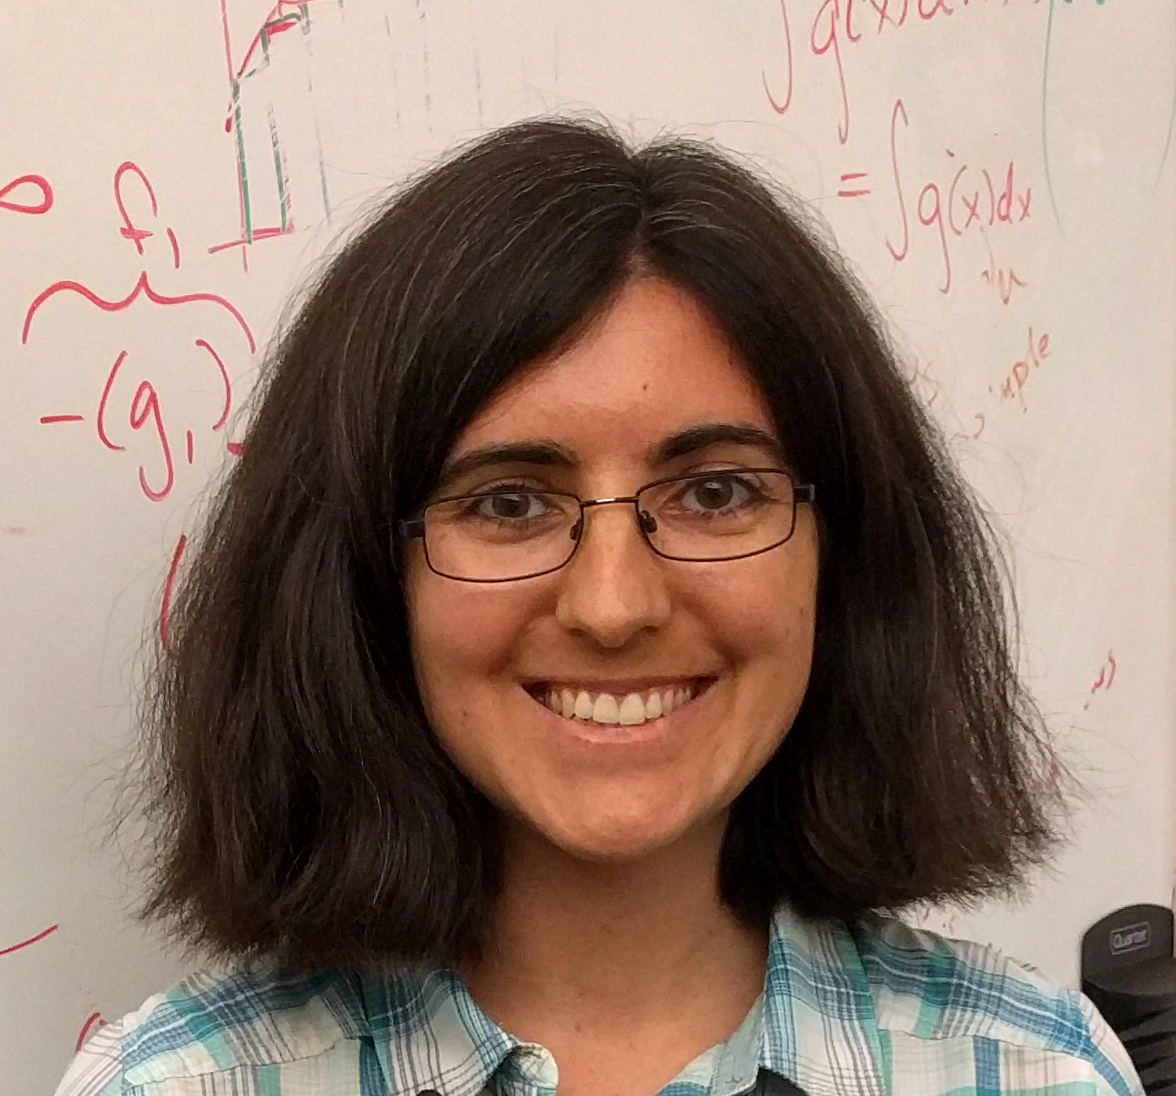
\includegraphics[height=2cm]{collaborators/tamara}
  			\caption*{Tamara Broderick \\ MIT}
  		\end{subfigure}\\
  	\end{figure}

\end{frame}

\begin{frame}{Our research problem}

Researchers often want to estimate the number of clusters present in a dataset. 
\vspace{-0.1in}
\pause
\begin{itemize}
\item[--] e.g., number of ancestral populations from DNA sequences; number of clusters from gene expressions; number of topics in a corpus. 
\end{itemize}

\pause

A Bayesian nonparametric (BNP) model makes inferring the number of clusters amenable to
Bayesian inference. We approximate the exact posterior using variational Bayes. 

\pause

\textbf{Question}: how sensitive is the VB approximation, and the resulting
inferences, to BNP model choices?

\pause 

\textbf{Problem}: re-running VB for multiple model choices is expensive. 

\pause 

\textbf{We propose}: a linear approximation to efficiently
estimate BNP sensitivity from a single run of VB (to avoid
expensive refitting). 

\end{frame}

\begin{frame}{Outline}
\begin{itemize}
\item {\bf The BNP Model}
\vspace{0.1in}

\item {\bf The Variational Approximation}
\vspace{0.1in}

\item {\bf Hyperparameter Sensitivity:} our linear approximation for VB sensitivity
\vspace{0.1in}

\item {\bf Results:} sensitivity to both parametric and functional perturbations
\vspace{0.1in}

\end{itemize}
\end{frame}

\begin{frame}{The BNP Model}
A {\bf Dirichlet process prior} allows for an infinite number of components. 
\vspace{-0.2in}
\begin{figure}[!h]
\centering
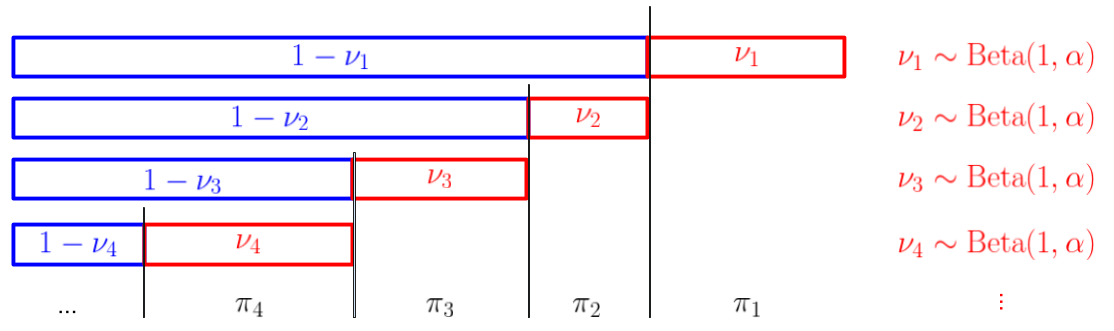
\includegraphics[width = 0.95\textwidth]{./figures/DP_stick_breaking.png}
\caption{A schematic of the Dirichlet process prior}
\end{figure}
\vspace{-0.2in}

While there are an infinite number of {\bf components}, there are a finite number of {\bf clusters} in a given dataset. \pause We might ask: 

\begin{enumerate}[(1)]
\item How many clusters are in the {\itshape current} dataset?

\pause 
\item Given our current knowledge, how many clusters would we expect to see in a {\itshape new} dataset?

\end{enumerate}

\pause 

These quantities depend on the choice of stick-breaking prior. 

\pause 

\begin{mdframed}[style=MyFrame]
\begin{center}
{\bf What makes this stick-breaking prior a reasonable one?}
\end{center}
\end{mdframed}

\end{frame}

\begin{frame}{The Variational Approximation}

Let $\theta$ be unknown parameters and $y$ the data. 

We posit a class of mean-field distributions parameterized by a real vector $\eta$. 

We solve
\begin{align*}
  \eta^* = \argmin_{\eta} KL\left(
      q(\theta \vert \eta )\big\| p(\theta | y)
      \right)
\end{align*}

\pause 

Note that 

\begin{itemize}
\item The optimal variational parameters $\eta^*$ depend on the prior through optimizing the KL objective. 

\pause 

\item The approximate posterior quantities are then functions of $\eta^*$, e.g.\
\begin{align*}
\eta^* \mapsto
\Expect_{q_{\eta^*}} \left[ \#\{\text{distinct clusters}\} \right]
\quad \text{ or } \quad
\eta^* \mapsto
\Expect_{q_{\eta^*}} 
\left[\#\{\substack{\text{distinct clusters}\\\text{in new dataset}}\} \right].
\end{align*}

\pause 

\end{itemize}

\begin{mdframed}[style=MyFrame]
\begin{center}
{\bf How do these approximate posterior quantities depend on the DP prior?}
\end{center}
\end{mdframed}

\end{frame}


\begin{frame}{Hyperparameter Sensitivity}

Let $\epsilon$ be a real-valued hyperparameter for the stick-breaking distribution
(e.\ g., this could be the $\alpha$ concentration parameter, or it could parameterize a functional shape).

\pause

{\bf Main idea: } We approximate the dependence of $\eta^*$ on $\epsilon$ with a first-order
Taylor expansion:

\begin{align*}
  \eta^*(\epsilon)  &\approx  \eta^*(0) +
  \frac{d \eta^*(\epsilon)}{d\epsilon^T}\Big|_{\epsilon=0} \epsilon
\end{align*}

\pause 

Notes: 
\begin{itemize}
\item Evaluation of the derivative can be done efficiently using formulas from Giordano et al. 2018 and auto-differentiation tools (Maclaurin et al. 2015).
 
\item We only use a linear approximation for the map $\epsilon \mapsto \eta^*(\epsilon)$. We retain nonlinearities in the map $\eta^* \mapsto
\Expect_{q_{\eta^*}} \left[ \#\{\text{distinct clusters}\} \right]$

\end{itemize}
\end{frame}

\begin{frame}{Results}

We use BNP to infer the number of species in iris dataset (Anderson 1936). 

\begin{figure}[!h]
\centering
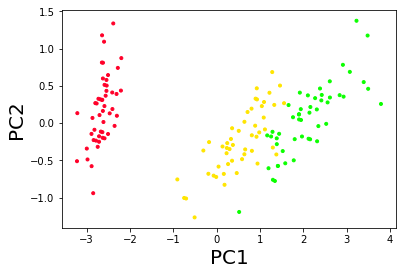
\includegraphics[width = 0.6\textwidth]{./images/iris_data.png}

\caption{The iris data projected onto the first two principal components. Color corresponds to the true iris species. }

\setlength{\textfloatsep}{-10pt}
\end{figure}

\end{frame}

%%%%%%%%%%
% Only refitted values 
\begin{frame}{Results: parametric sensitivity}

\begin{figure}
\centering
\begin{knitrout}
\definecolor{shadecolor}{rgb}{0.969, 0.969, 0.969}\color{fgcolor}

{\centering 
\includegraphics[width=0.98\linewidth,height=0.294\linewidth]{masked_results_fig/param_sens_plot_thresh_0_masked1-1} 

}



\end{knitrout}
\begin{knitrout}
\definecolor{shadecolor}{rgb}{0.969, 0.969, 0.969}\color{fgcolor}

{\centering 
\includegraphics[width=0.98\linewidth,height=0.294\linewidth]{masked_results_fig/param_sens_plot_thresh_0b_masked-1} 

}



\end{knitrout}
\end{figure}

\end{frame}

%%%%%%%%%%
% Refitted and LR 
\begin{frame}{Results: parametric sensitivity}

\begin{figure}
\centering
\begin{knitrout}
\definecolor{shadecolor}{rgb}{0.969, 0.969, 0.969}\color{fgcolor}

{\centering 
\includegraphics[width=0.98\linewidth,height=0.294\linewidth]{masked_results_fig/param_sens_plot_thresh_0_masked1-2} 

}



\end{knitrout}
\begin{knitrout}
\definecolor{shadecolor}{rgb}{0.969, 0.969, 0.969}\color{fgcolor}

{\centering 
\includegraphics[width=0.98\linewidth,height=0.294\linewidth]{masked_results_fig/param_sens_plot_thresh_0b_masked-1} 

}



\end{knitrout}
\end{figure}

\end{frame}

%%%%%%%%%%%%%%%%%%%
% first row
\begin{frame}{Results: parametric sensitivity}

\begin{figure}
\centering
\begin{knitrout}
\definecolor{shadecolor}{rgb}{0.969, 0.969, 0.969}\color{fgcolor}

{\centering 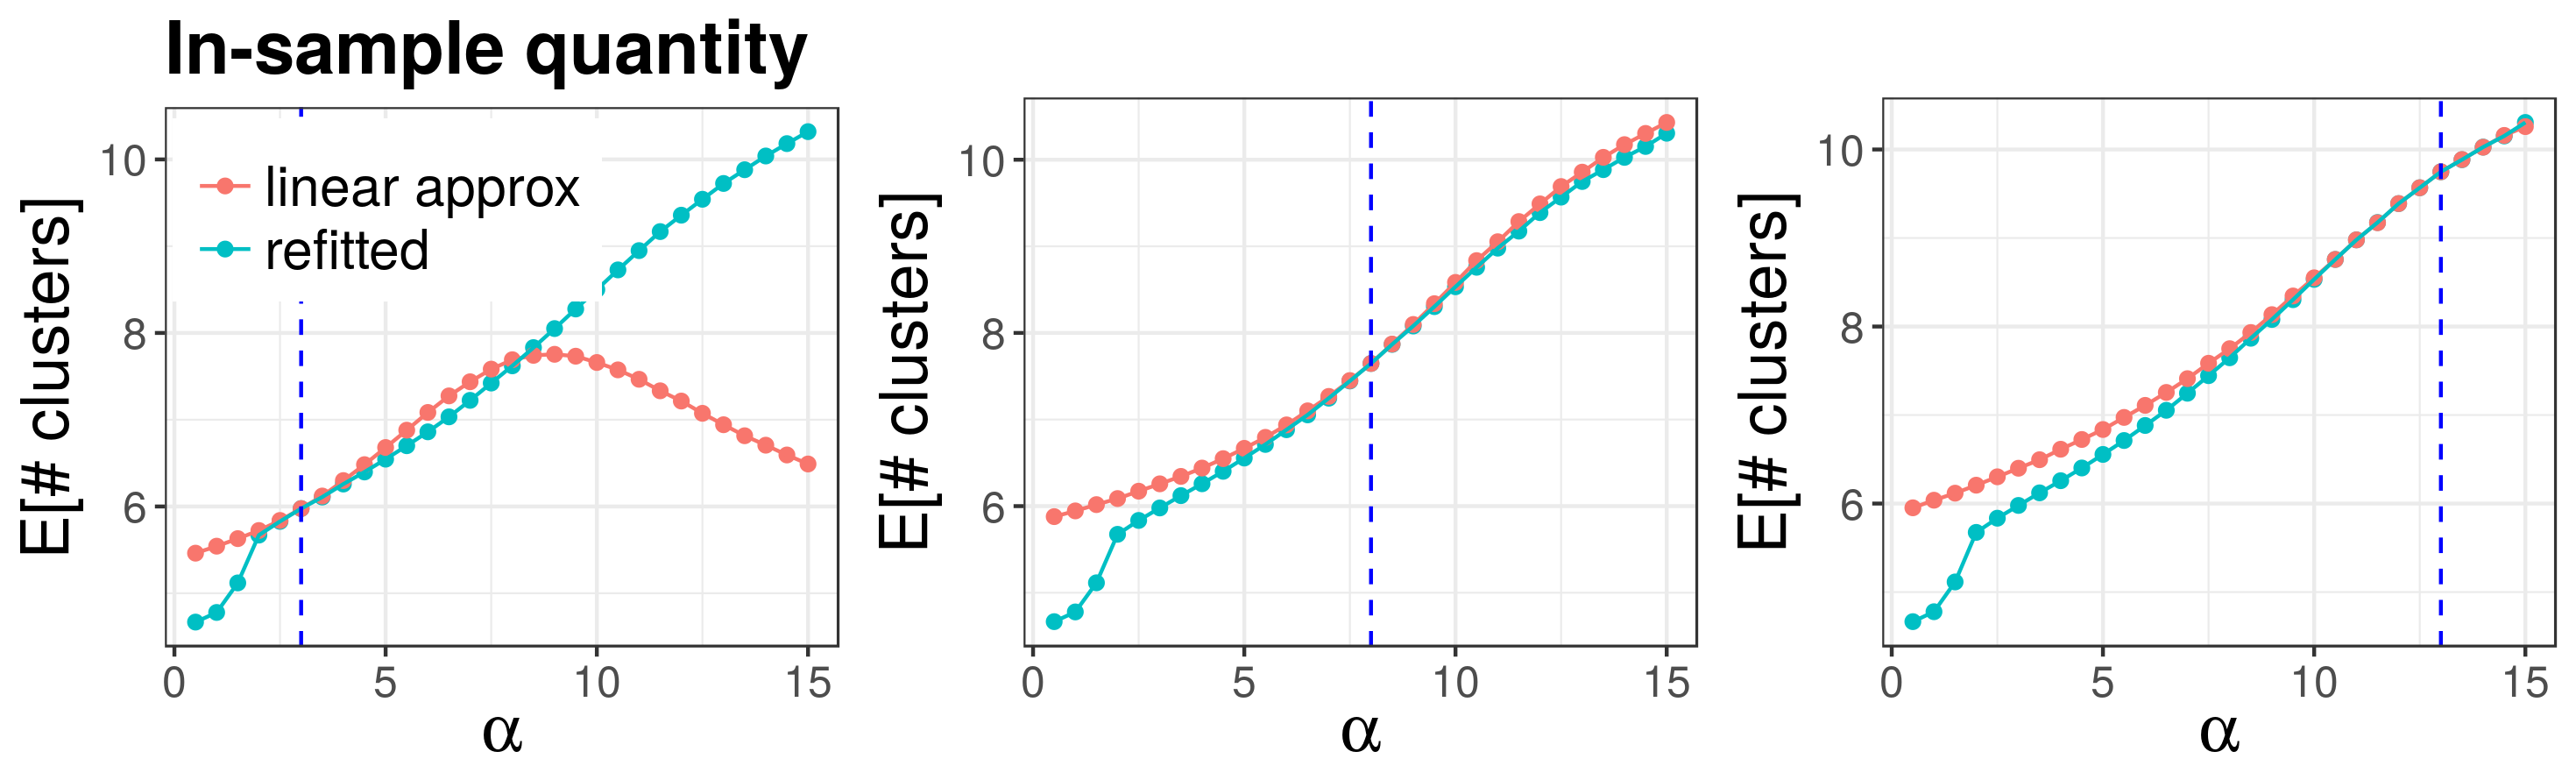
\includegraphics[width=0.98\linewidth,height=0.294\linewidth]{figure/param_sens_plot_thresh_0-1} 

}



\end{knitrout}
\begin{knitrout}
\definecolor{shadecolor}{rgb}{0.969, 0.969, 0.969}\color{fgcolor}

{\centering 
\includegraphics[width=0.98\linewidth,height=0.294\linewidth]{masked_results_fig/param_sens_plot_thresh_0b_masked-1} 

}



\end{knitrout}
% \caption{Comparison of in-sample (top) and predictive (bottom) expected number of clusters computed by re-optimizing versus the linear approximation. 
% The blue vertical line indicates the location of $\alpha_0$}
\end{figure}


\end{frame}


\begin{frame}{Results: parametric sensitivity}

\begin{figure}
\centering
\begin{knitrout}
\definecolor{shadecolor}{rgb}{0.969, 0.969, 0.969}\color{fgcolor}

{\centering 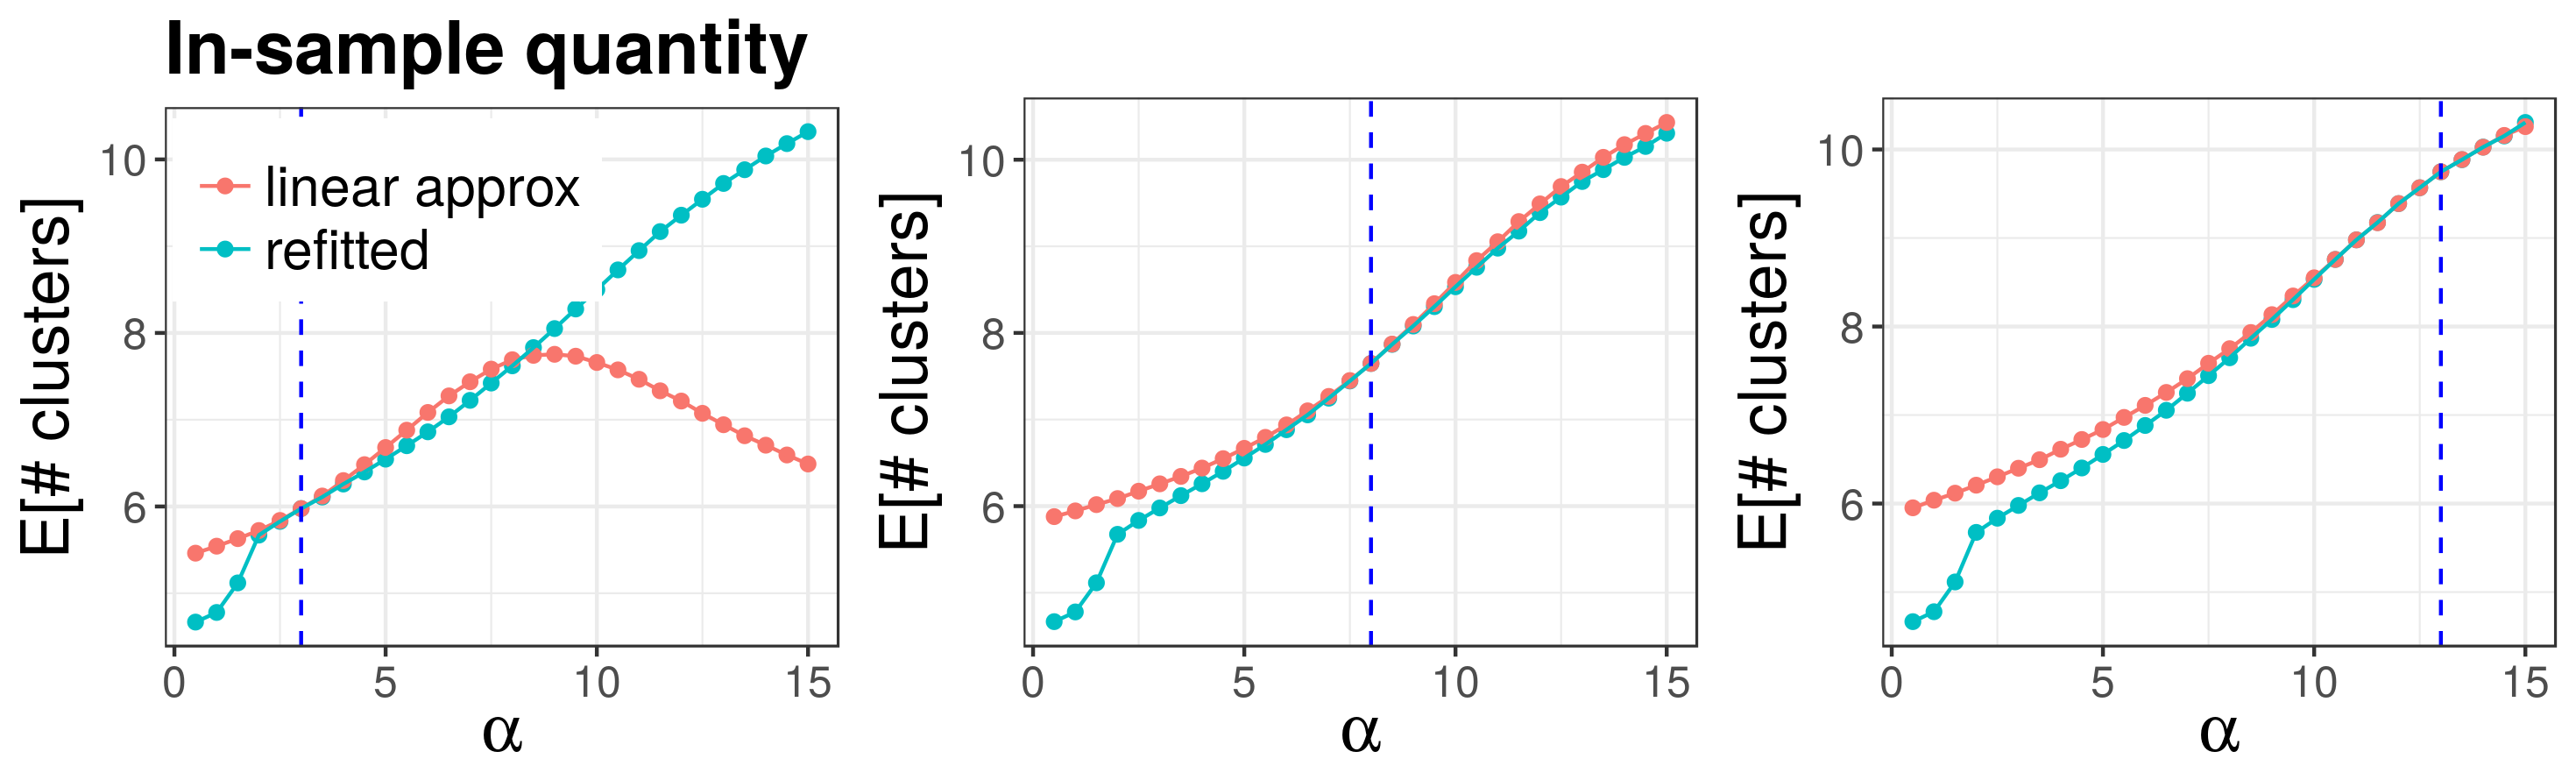
\includegraphics[width=0.98\linewidth,height=0.294\linewidth]{figure/param_sens_plot_thresh_0-1} 

}



\end{knitrout}
\begin{knitrout}
\definecolor{shadecolor}{rgb}{0.969, 0.969, 0.969}\color{fgcolor}

{\centering 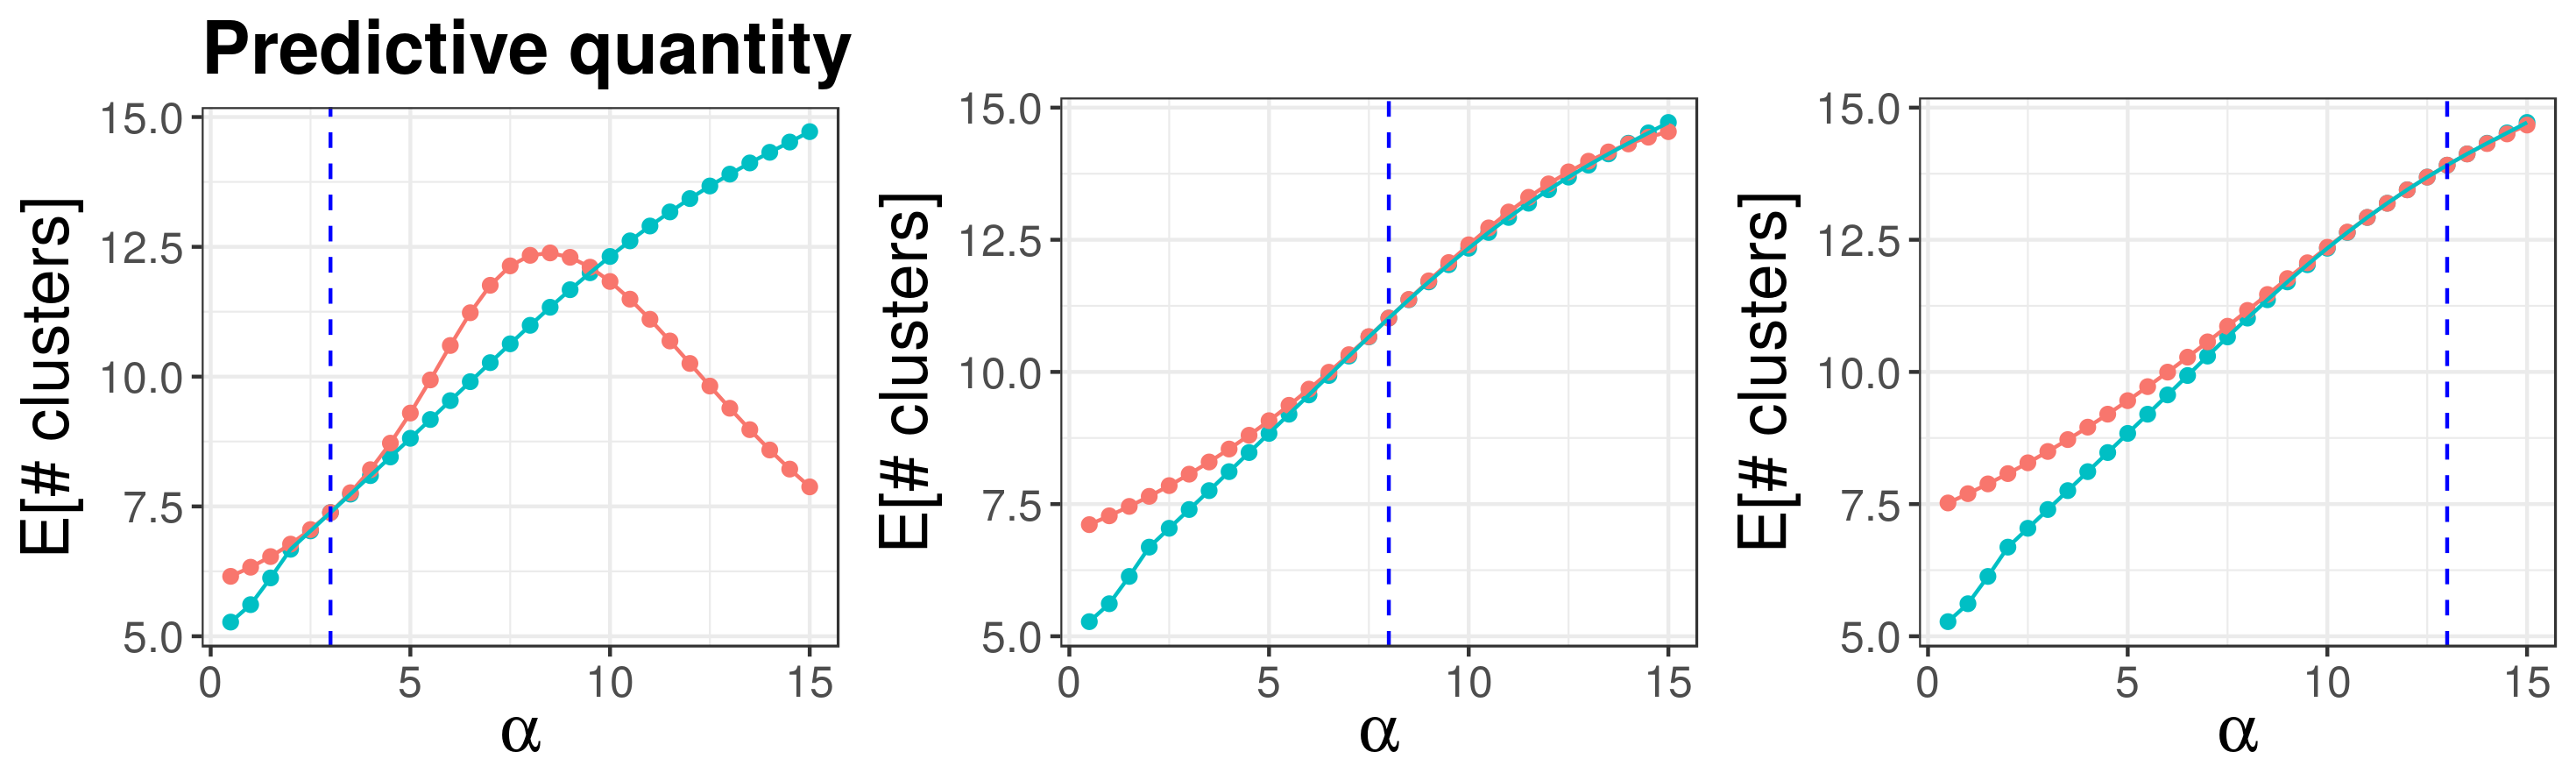
\includegraphics[width=0.98\linewidth,height=0.294\linewidth]{figure/param_sens_plot_thresh_0b-1} 

}



\end{knitrout}
% \caption{Comparison of in-sample (top) and predictive (bottom) expected number of clusters computed by re-optimizing versus the linear approximation. 
% The blue vertical line indicates the location of $\alpha_0$}
\end{figure}

\end{frame}

\begin{frame}{Results: functional perturbation}
% Now consider a multiplicative perturbation $\phi$ to
% the original beta distribution $p_0$ for the stick-breaking proportions:
% %
% \begin{align*}
% \label{eq:expon_perturb}
% 	p_c(\nu_k \vert \delta, \phi) :=
%   \frac{p_{0}(\nu_k)\phi(\nu_k)^\delta}
%        {\int_0^1 p_0(\nu_k')\phi(\nu')^\delta d\nu_k'}.
% \end{align*}
% \pause 
Suppose we wish to replace the original beta prior $p_0$ with another distribution $p_1$. Then we set our perturbation to be
\begin{align*}
p_c(\nu_k \vert \delta) \propto p_{0}(\nu_k)\left(\frac{p_1(\nu_k)}{p_0(\nu_k)}\right)^\delta
\end{align*}
\vspace{-0.25in}
\begin{figure}[!h]
\centering
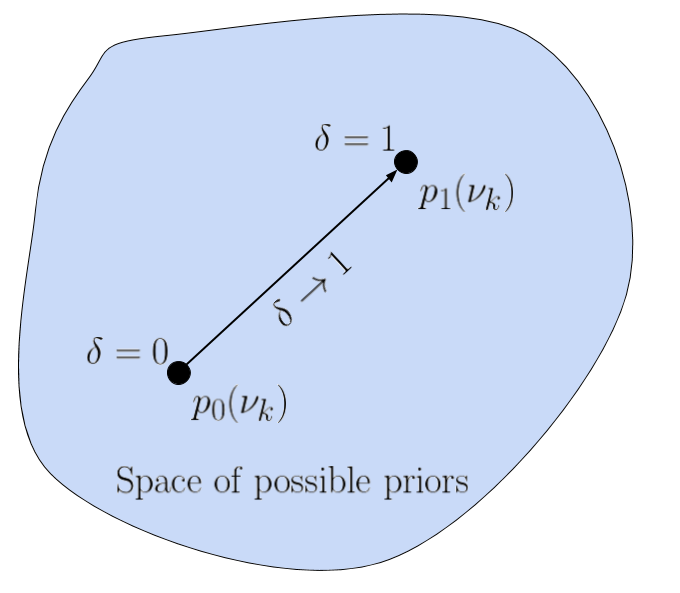
\includegraphics[width = 0.65\textwidth]{./images/functional_perturbation.png}
\setlength{\textfloatsep}{-10pt}
\end{figure}

\end{frame}

\begin{frame}{Results: functional perturbation}
\begin{figure}
\centering
\begin{knitrout}
\definecolor{shadecolor}{rgb}{0.969, 0.969, 0.969}\color{fgcolor}
{\centering 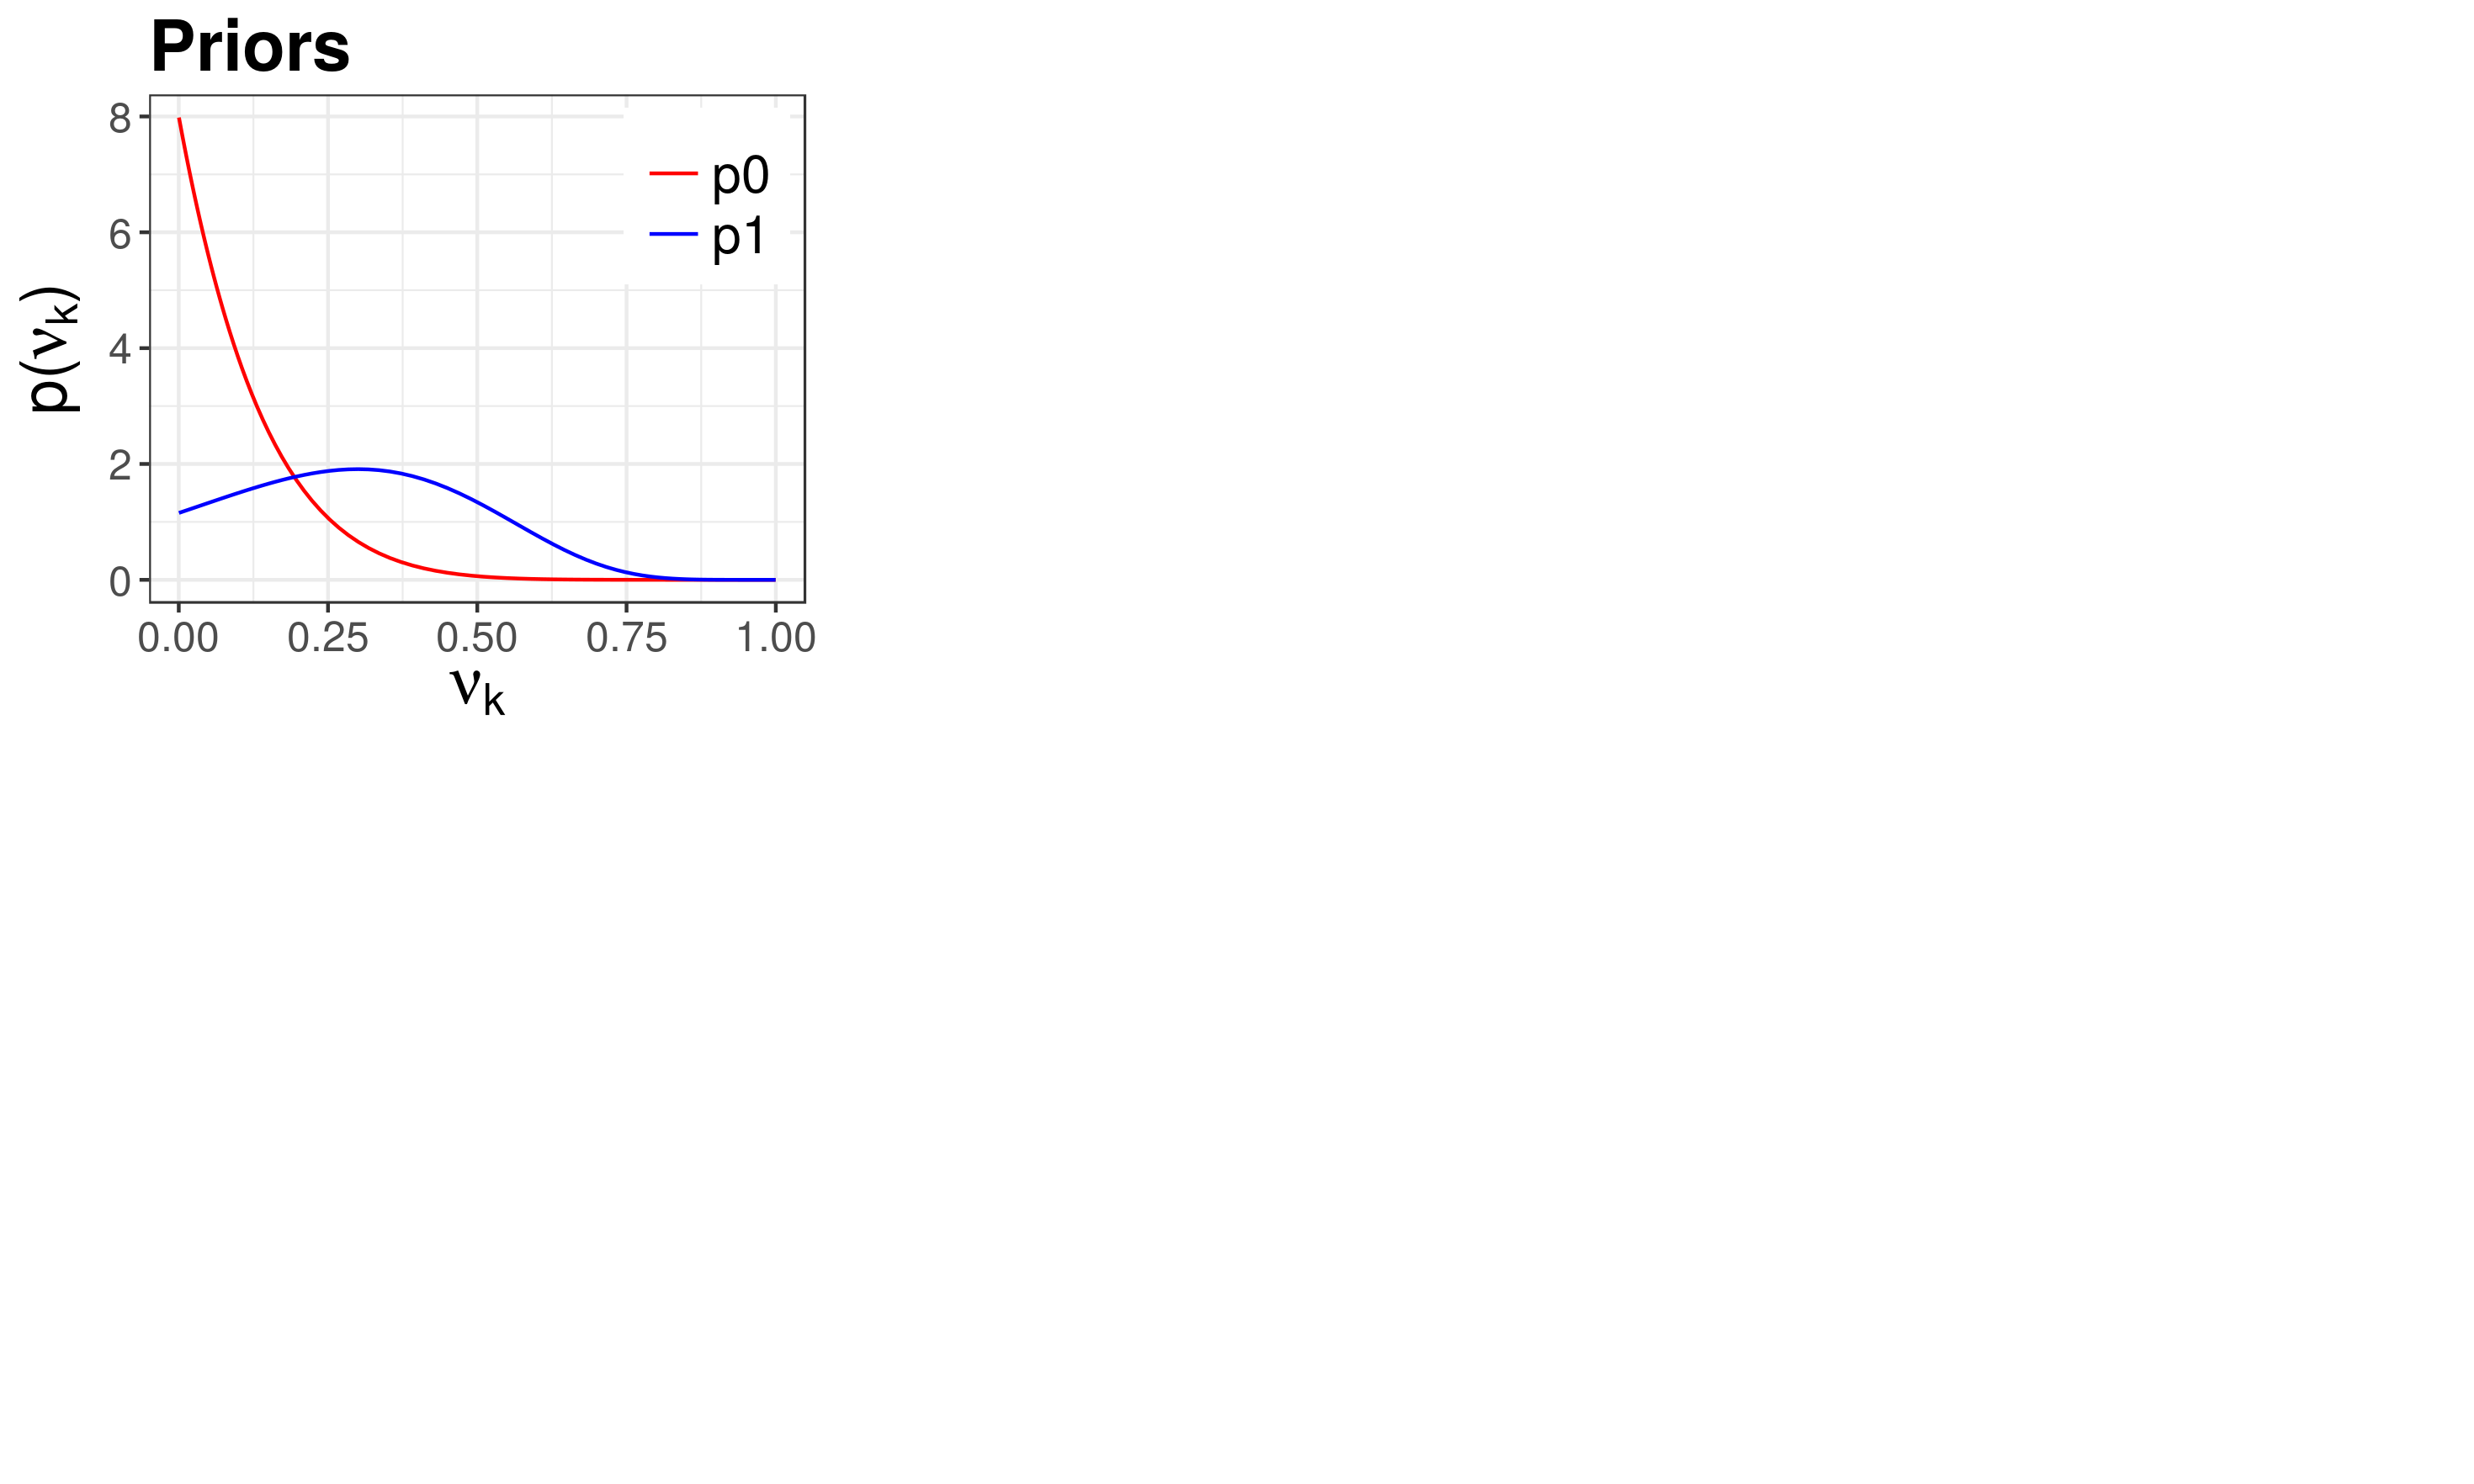
\includegraphics[width=0.98\linewidth,height=0.588\linewidth]{masked_results_fig/fun_sens_masked_1} 
}
\end{knitrout}
\end{figure}
\end{frame}

\begin{frame}{Results: functional perturbation}
\begin{figure}
\centering
\begin{knitrout}
\definecolor{shadecolor}{rgb}{0.969, 0.969, 0.969}\color{fgcolor}
{\centering 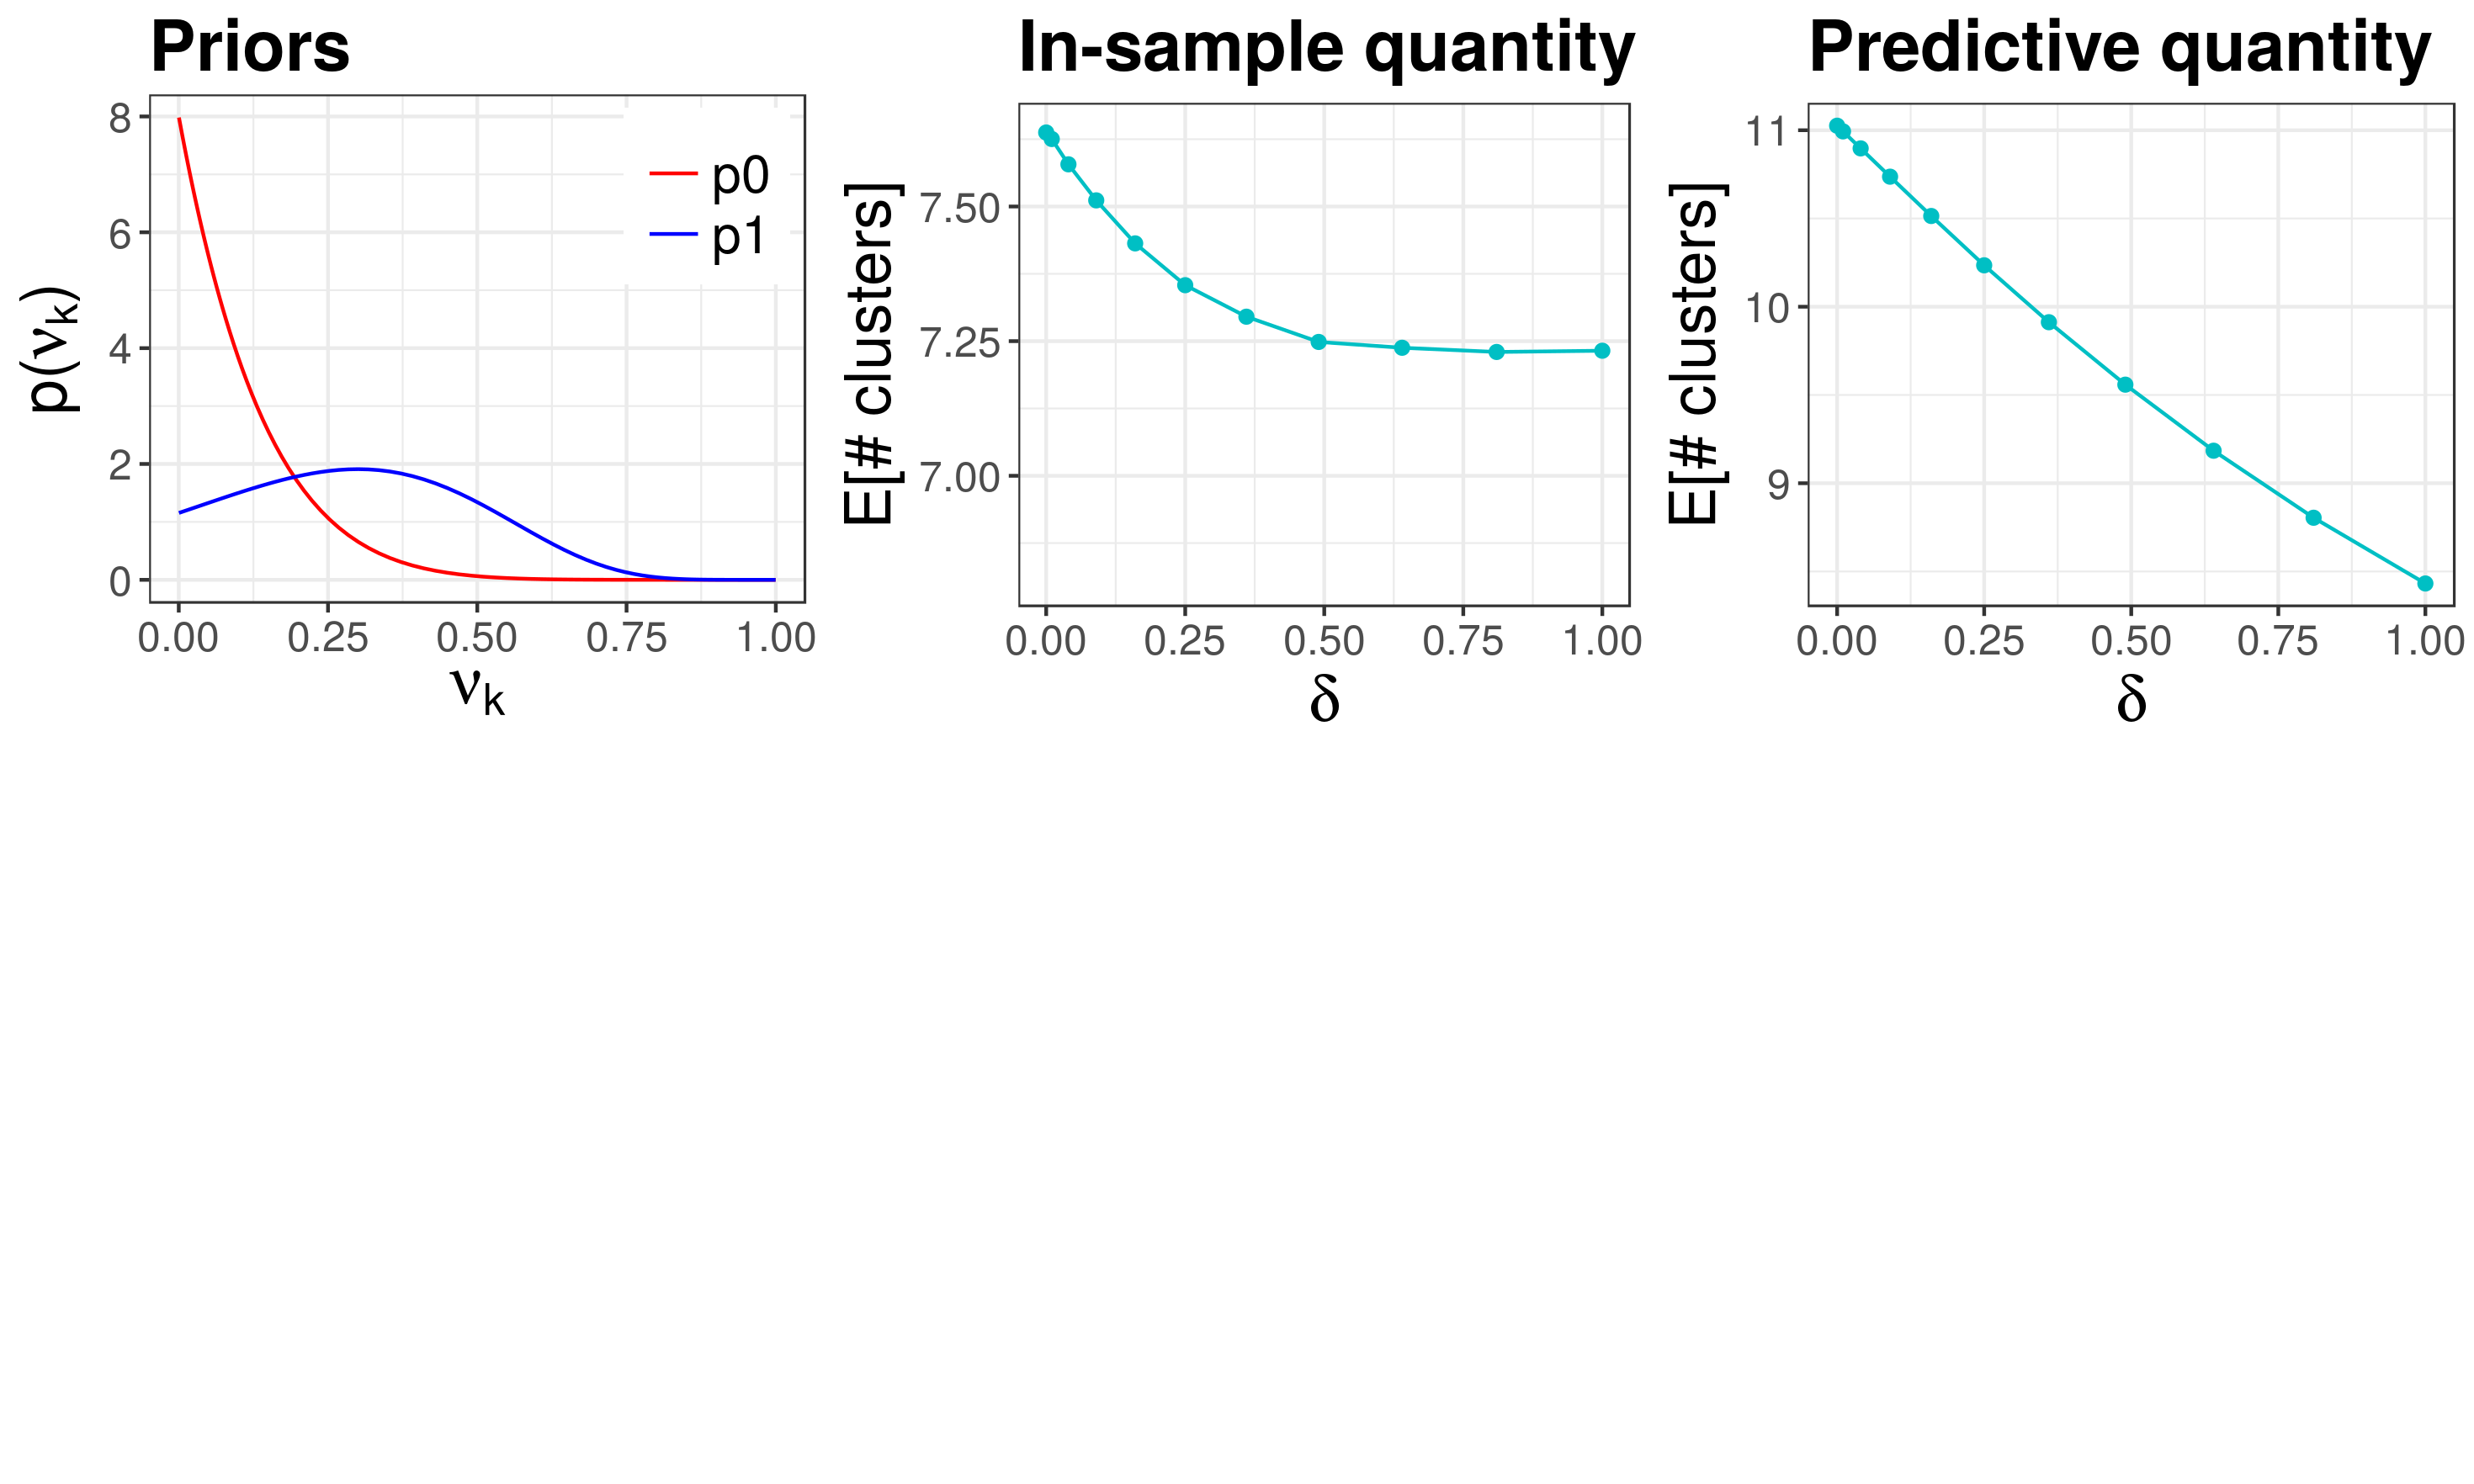
\includegraphics[width=0.98\linewidth,height=0.588\linewidth]{masked_results_fig/fun_sens_masked_2} 
}
\end{knitrout}
\end{figure}
\end{frame}

\begin{frame}{Results: functional perturbation}
\begin{figure}
\centering
\begin{knitrout}
\definecolor{shadecolor}{rgb}{0.969, 0.969, 0.969}\color{fgcolor}
{\centering 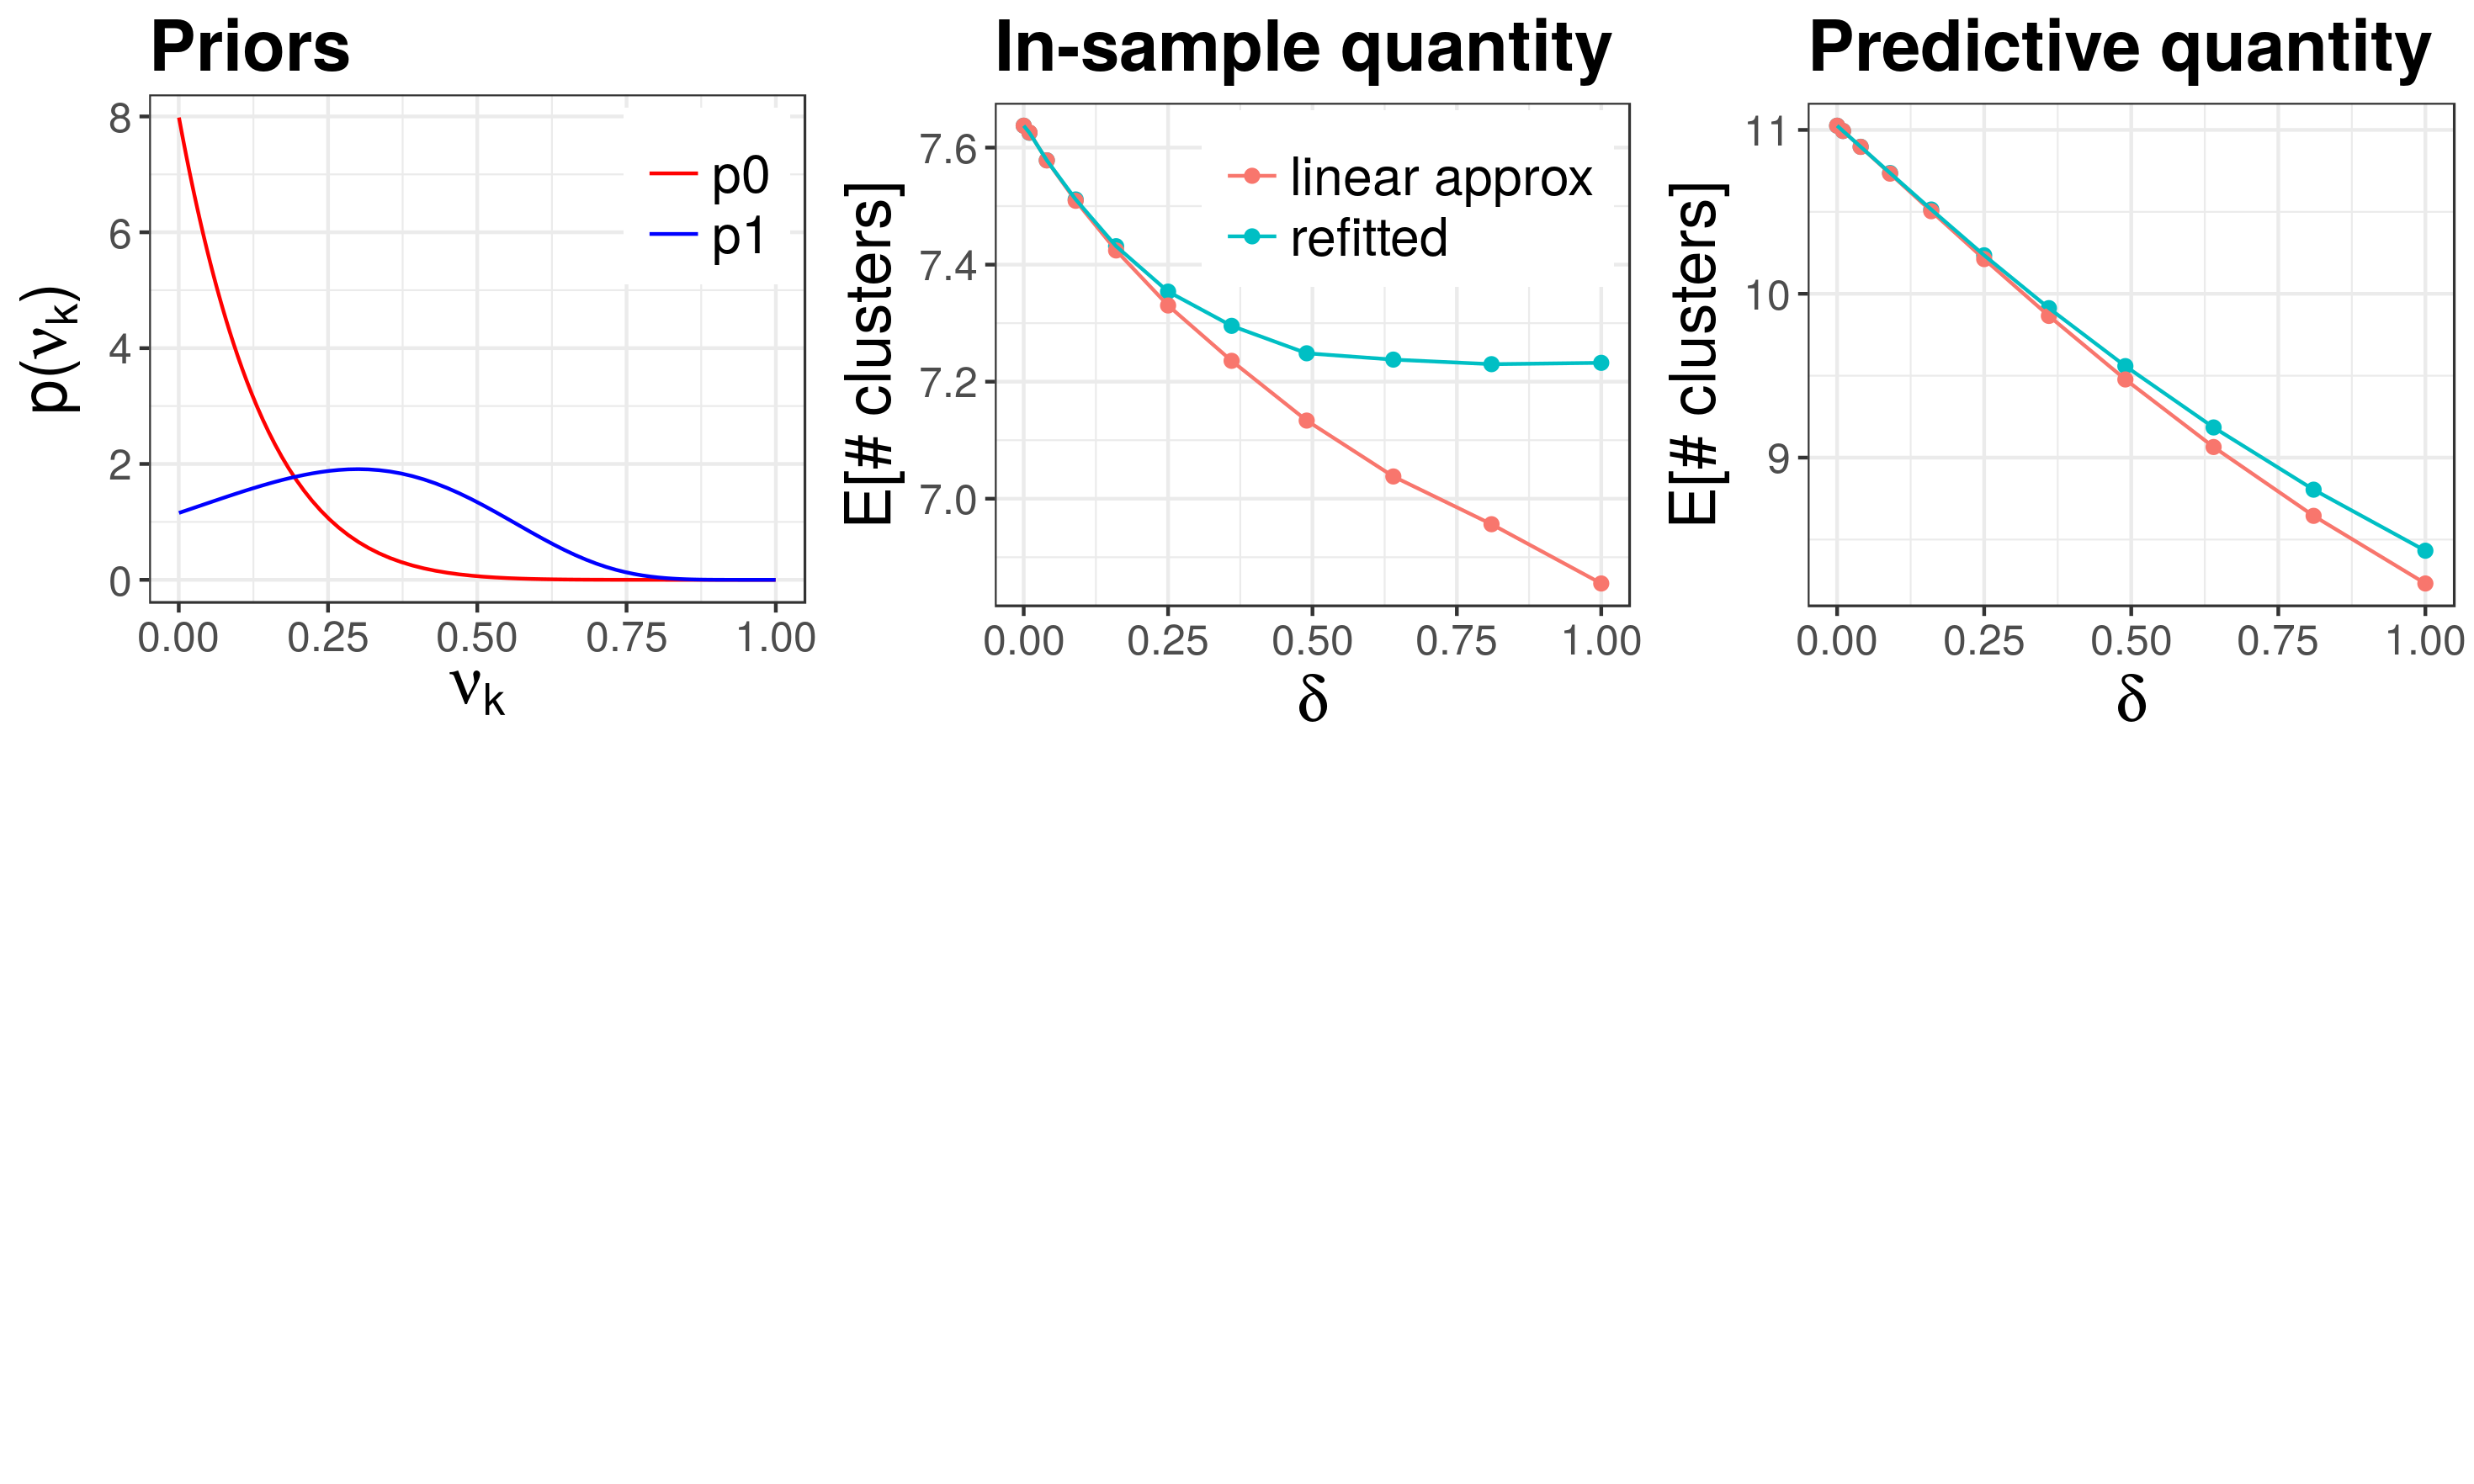
\includegraphics[width=0.98\linewidth,height=0.588\linewidth]{masked_results_fig/fun_sens_masked_3} 
}
\end{knitrout}
\end{figure}
\end{frame}

% \begin{frame}{Results: functional perturbation}
% \begin{figure}
% \centering
% <<foo3, cache=cache_knitr>>=
% SetImageSize(aspect_ratio= 2.0 * base_aspect_ratio)
% @
% <<foo, cache=cache_knitr, fig.show='hold'>>=
% source("Rscripts/appendix_functional_sens_results_thresh0_masked.R", echo=knitr_debug, print.eval=TRUE)
% @
% \end{figure}
% 
% \end{frame}

\begin{frame}{Results: functional perturbation}
\begin{figure}
\centering

\begin{knitrout}
\definecolor{shadecolor}{rgb}{0.969, 0.969, 0.969}\color{fgcolor}

{\centering 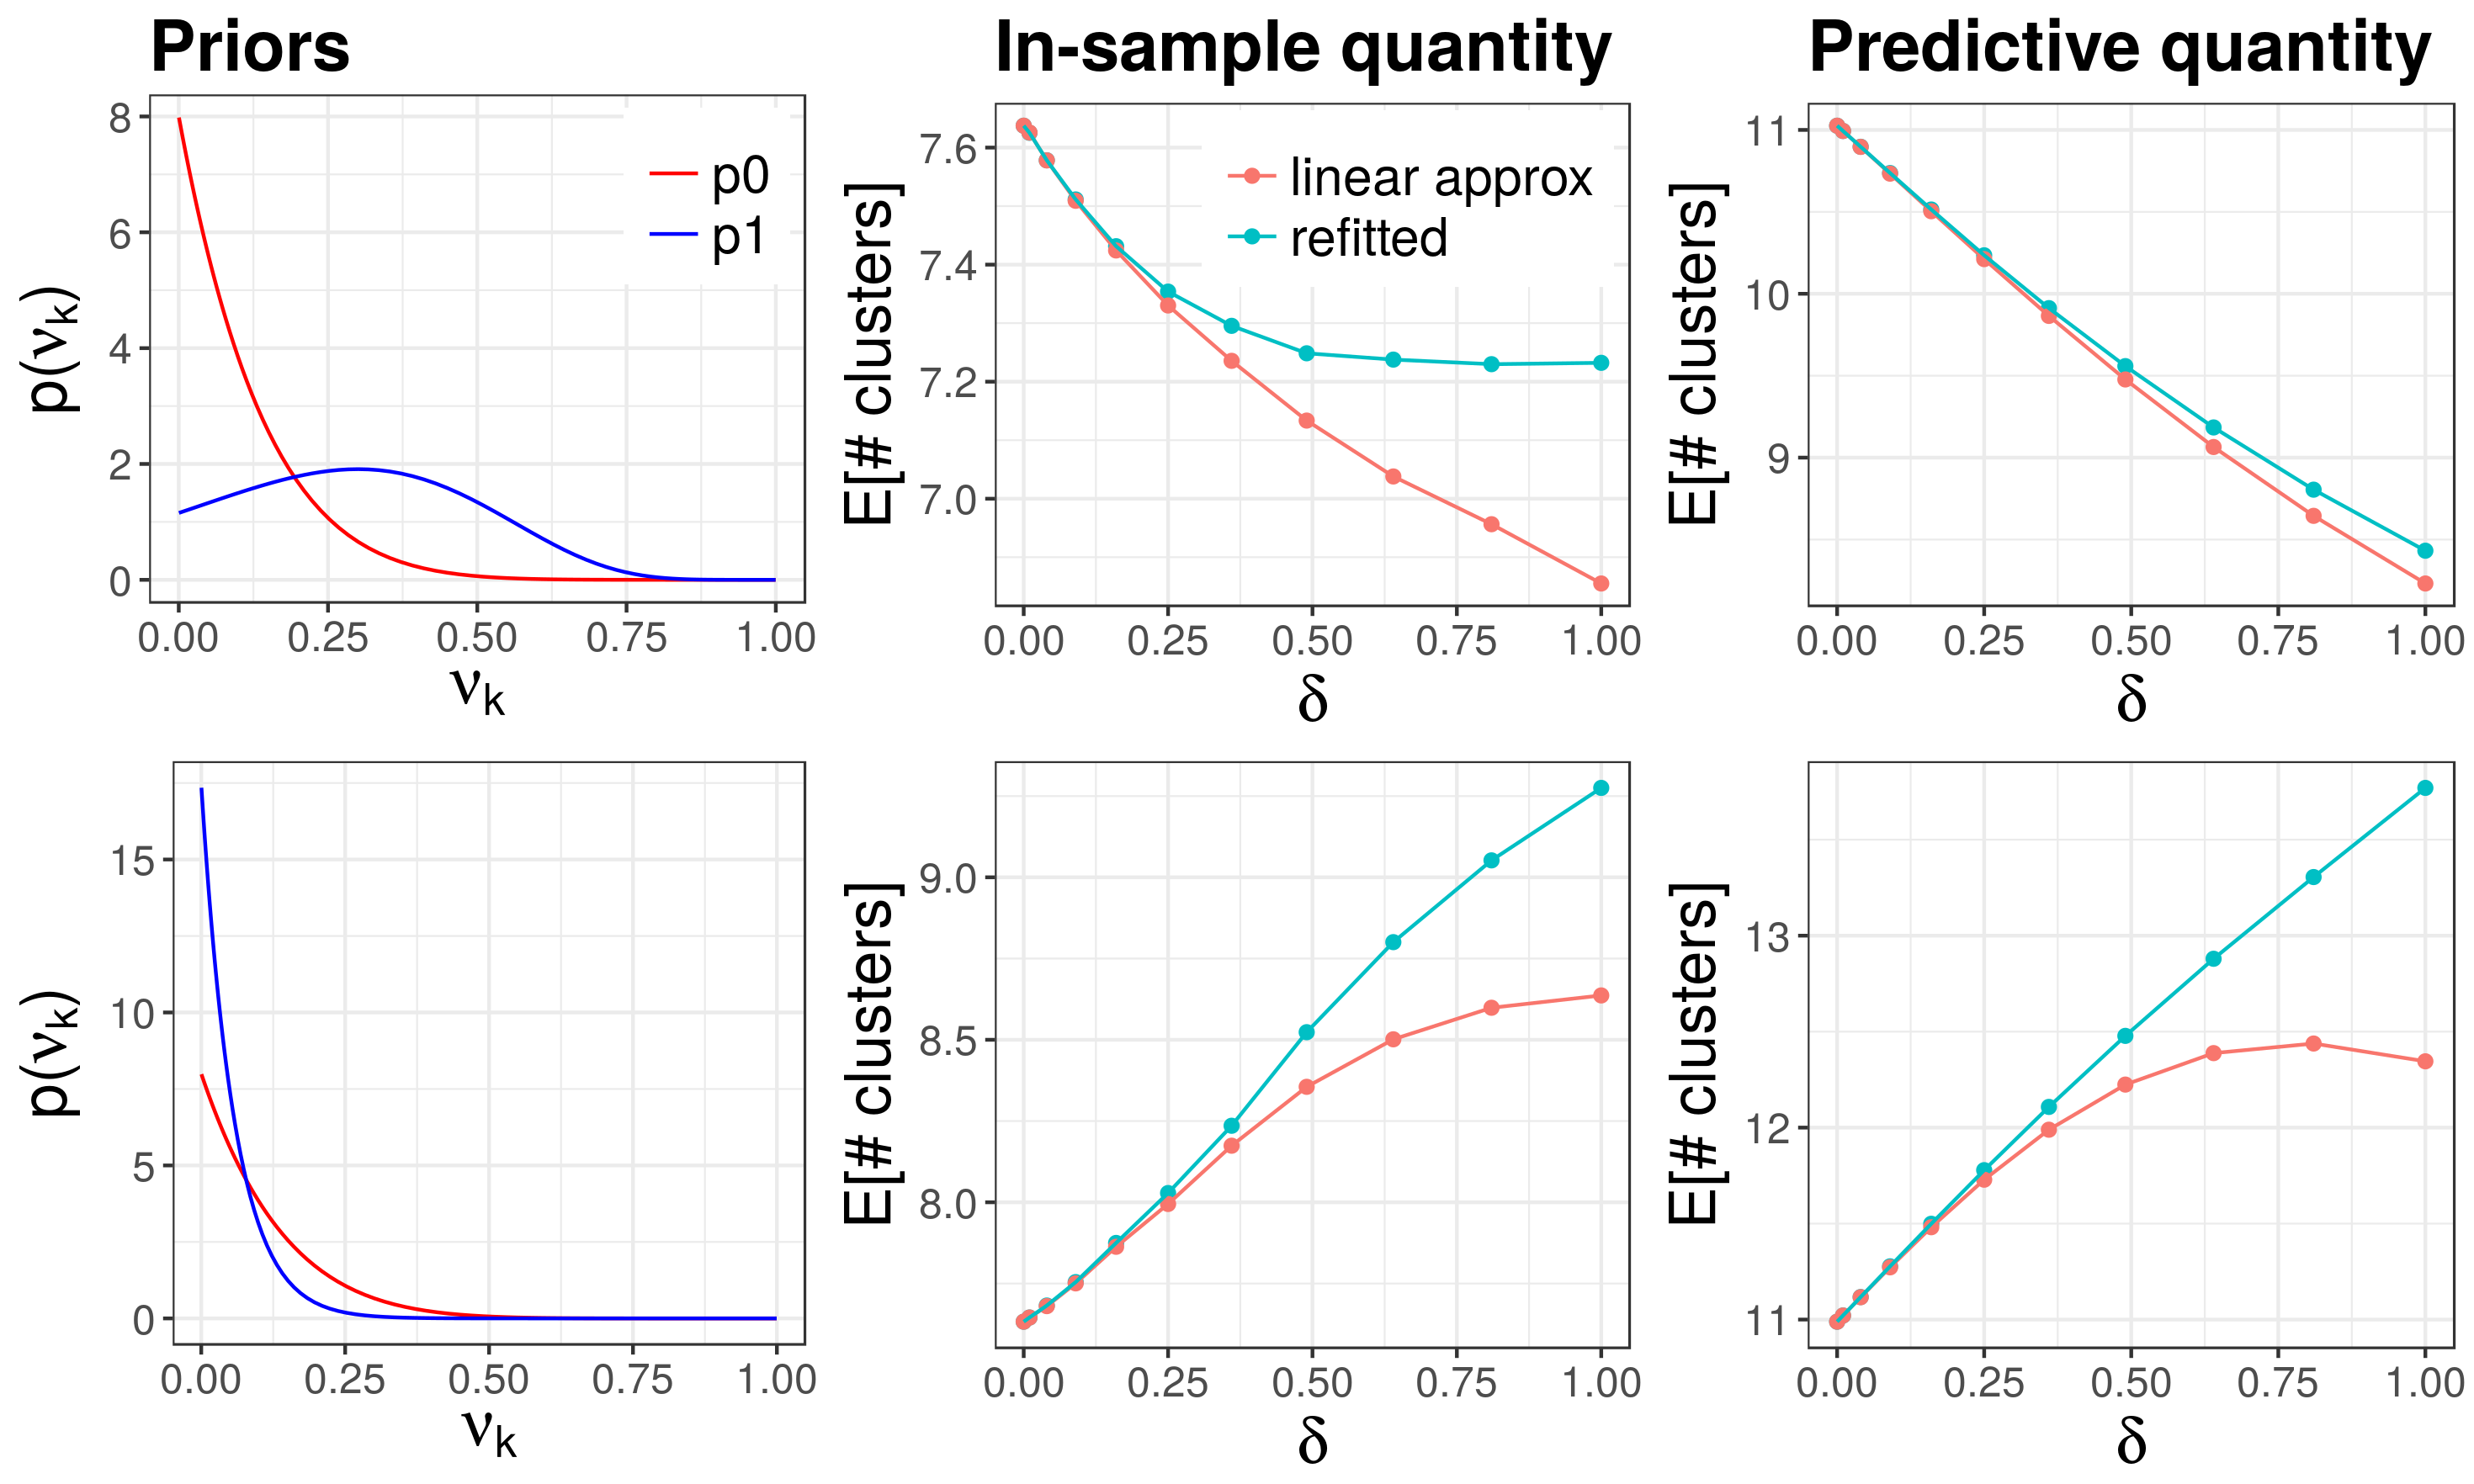
\includegraphics[width=0.98\linewidth,height=0.588\linewidth]{figure/functional_sens_plot_thresh0-1} 

}



\end{knitrout}
\end{figure}

\end{frame}


\begin{frame}{Summary}

{\bf Next steps}
\begin{itemize}
\item Higher order Taylor-expansions
\pause 
\item Other forms of functional perturbations
\pause 
\item Other metrics for ``number of clusters"
\pause
\item Issues with multiple optima
\pause 
\end{itemize}
\vspace{0.2in}

\begin{mdframed}[style=MyFrame]
\begin{center}
{\bf In summary, our linear approximation provides a fast and reasonable alternative to re-evaluating the full model after changing the BNP prior.}
\end{center}
\end{mdframed}

\end{frame}

\begin{frame}

{\bf For more, see our paper: }\newline
Runjing Liu, Ryan Giordano, Michael I. Jordan, Tamara Broderick. \newline
“Evaluating Sensitivity to the Stick Breaking Prior in Bayesian Nonparametrics.” \newline {\color{blue}\url{https://arxiv.org/pdf/1810.06587.pdf}}

{\bf And our code: }\newline
Paragami: library for sensitivity analysis in optimization problems \newline
{\color{blue}\url{https://github.com/rgiordan/paragami}}

Code to evaluate BNP sensitivity implemented for this talk: 
{\color{blue}\url{https://github.com/Runjing-Liu120/sensitivity_to_stick_breaking_in_BNP}}

\vspace{0.2in}

\begin{scriptsize}

{\bf References}

E. Anderson. The species problem in iris. {\itshape Annals of the Missouri Botanical Garden}, 23(3):457–509, 1936.

R. Giordano, T. Broderick, and M. I. Jordan. Covariances, robustness, and variational Bayes. {\itshape Journal of Machine Learning Research}, 19(51):1–49, 2018.

D. Maclaurin, D. Duvenaud, and R. P. Adams. Autograd: Effortless gradients in numpy. {\itshape In International Conference on Machine Learning 2015 AutoML Workshop}, 2015.

\end{scriptsize}

\end{frame}


\end{document}
